\documentclass[a4paper,norsk, 10pt]{article}
\usepackage[utf8]{inputenc}
\usepackage{verbatim}
\usepackage{listings}
\usepackage{graphicx}
\usepackage[norsk]{babel}
\usepackage{a4wide}
\usepackage{color}
\usepackage{amsmath}
\usepackage{float}
\usepackage{amssymb}
\usepackage[dvips]{epsfig}
\usepackage[toc,page]{appendix}
\usepackage[T1]{fontenc}
\usepackage{cite} % [2,3,4] --> [2--4]
\usepackage{shadow}
\usepackage{hyperref}
\usepackage{titling}
\usepackage{marvosym }
\usepackage{subcaption}
\usepackage[noabbrev]{cleveref}
\usepackage{cite}
\usepackage{todonotes}


\setlength{\droptitle}{-10em}   % This is your set screw

\setcounter{tocdepth}{2}

\lstset{language=c++}
\lstset{alsolanguage=[90]Fortran}
\lstset{alsolanguage=Python}
\lstset{basicstyle=\small}
\lstset{backgroundcolor=\color{white}}
\lstset{frame=single}
\lstset{stringstyle=\ttfamily}
\lstset{keywordstyle=\color{red}\bfseries}
\lstset{commentstyle=\itshape\color{blue}}
\lstset{showspaces=false}
\lstset{showstringspaces=false}
\lstset{showtabs=false}
\lstset{breaklines}
\title{AST4320 Oblig2}
\author{Daniel Heinesen, daniehei}
\begin{document}
\maketitle

\section{1}
\subsection{a)}

To find the mean molecular weight if the intergalactic medium (IGM) we use that
\begin{equation}
\dfrac{1}{\mu} = \sum_i \dfrac{X_i}{A_i} = 2X + 4/3\cdot Y,
\end{equation}
where $X_i$ is the fraction of species $i$ and $A_i$ is the atomic mass of said species divided by the total number of particles it ionizes to. For the IGM we have a fraction of hydrogen $X = 0.76$ and a fraction of helium $Y = 0.24$, giving us

\begin{equation}
\mu = \dfrac{1}{2\cdot0.76 + 4/3\cdot0.24} = 0.59.
\end{equation}

\subsection{b)}
The Jeans length is given as 

\begin{equation}
\lambda_j = c_s\left(\dfrac{\pi}{G\rho}\right)^{1/2},
\end{equation}
where the speed of sound $c_s$ for a gas is given as
\begin{equation}
c_s = \sqrt{\dfrac{k_b T}{\mu m_p}} = 11.83 \text{m/s}.
\end{equation}
We are using that $T=10^4$ K. We have to find the pressure of the IGM. For this we assume that the gas only have baryonic matter, so
\begin{equation}
\rho = \rho_b(1+z)^3 = \Omega_b \rho_c (1+z)^3,
\end{equation}
where $\Omega_b = 0.049$ and $\rho_c = 9.47\cdot 10^{-27}$ g/cm$^{3}$. 
We then see that get
\begin{equation}
\lambda_j(z) = 3.9\text{ Mpc}\cdot(1+z)^{-3/2}.
\end{equation}
This gives $k$

\begin{equation}
k = \dfrac{2\pi}{\lambda_j(z)} = 1.61 \text{ Mpc}^{-1} (1+z)^{3/2}.
\end{equation}

\subsection{c)}
We can use Hubble's law to find the different in velocity across the Jeans length of the IGM, thereby giving us the velocity width. Through Hubble's law we get

\begin{equation}
\Delta v = H(z) \lambda_j,
\end{equation}
where
\begin{equation}
H(z) = H_0 (\Omega_m(1+z)^3 + \Omega_r(1+z)^4 + \Omega_{\Lambda})^{1/2}.
\end{equation}

This gives us that

\begin{equation}
\Delta v = H_0 (\Omega_m(1+z)^3 + \Omega_r(1+z)^4 + \Omega_{\Lambda})^{1/2}3.9\text{ Mpc}\cdot(1+z)^{-3/2} 
\end{equation}
\begin{equation}
= 264.5 \text{ km/s}\cdot (\Omega_m + \Omega_r(1+z) + \Omega_{\Lambda}(1+z)^{-3})^{1/2} = 264.5 \text{ km/s}\cdot (0.308 +  0.692(1+z)^{-3})^{1/2}
\end{equation}


\subsection{d)}

\todo{See over this!} 

\subsection{e)}

The thermal broadening scale is given as

\begin{equation}
 v_{th} = \sqrt{\dfrac{2k_b T}{m_p}},
 \end{equation} 
where $T = 10^4$ K. This gives us
\begin{equation}
v_{th} = 12.85 \text{ km/s},
\end{equation}
which is an order small that all values of $z$.

\section{Exercise 2}

We would like to find the optical depth $\tau_e$ of the IGM as a function of redshift $z$. The optical depth is given as

\begin{equation}\label{eq:tau}
\tau_e(z) = c\int_0^z \frac{n_e(z) \sigma_T dz}{H(z)(1+z)},
\end{equation}
where $\sigma_t$ is the Thompson cross section, $n_e$ the electron density and $H(z)$ the Hubble parameter. Since the Universe is taken to be completely ionized, he assume that $n_e \approx \bar{n_H} = 1.9 \cdot 10^{-7} (1+z)^3 $ cm$^{-3}$. We get the Hubble parameter from the Friedmann equation

\begin{equation}
H(z) = H_0 \sqrt{\Omega_m (1+z)^3 + \Omega_r(1+z)^4 + \Omega_{\Lambda}},
\end{equation}
where $\Omega_{\Lambda} = 0.692$, $\Omega_m = 0.308$ and $\Omega_r = 0$.

We will integrate \eqref{eq:tau} from $z=0$ to $10$. We assume that $\tau_e(0) \approx 0$.


\begin{figure}[H]
\centering
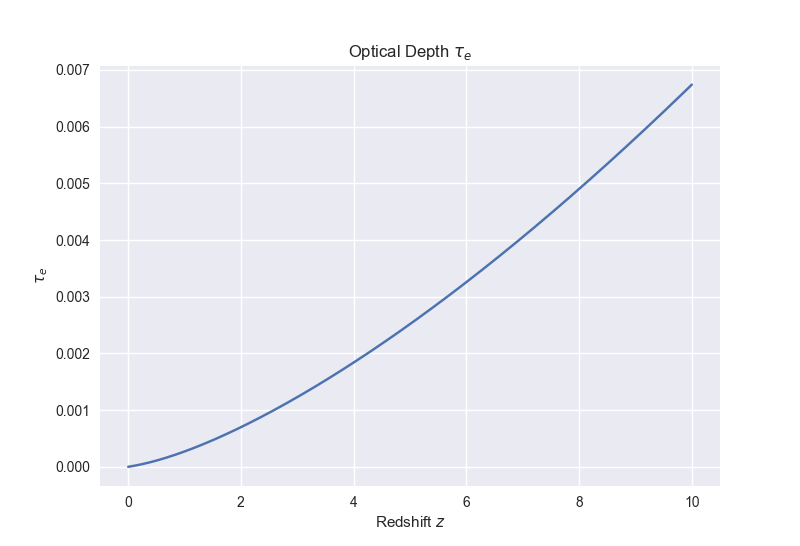
\includegraphics[scale=0.7]{tau}
\caption{The optical depth of the intergalactic medium. We see that for larger redshift the optical depth increases.}
\end{figure}


\section{Exercise 3}
\subsection{a)}
We have the differential equation for an isothermal halo

\begin{equation}\label{eq:diff}
-\dfrac{k_b T}{m_{DM} r^2}\dfrac{d}{dr}r^2 \dfrac{d}{dr} \ln \rho = 4 \pi G\rho.
\end{equation}

We have an ansatz that
\begin{equation}\label{eq:ansatz}
\rho(r) = \dfrac{A}{r^2}, \qquad A = \frac{k_b T}{2\pi Gm_{DM}}.
\end{equation}

To see that this is a solution, we put \eqref{eq:ansatz} into \eqref{eq:diff}. Looking at the RHS of \eqref{eq:diff} we get 


\begin{equation}
-\dfrac{k_b T}{m_{DM} r^2}\dfrac{d}{dr}r^2 \dfrac{d}{dr} \ln \rho = -\dfrac{k_b T}{m_{DM} r^2}\dfrac{d}{dr}r^2 \dfrac{r^2}{A}\cdot \left(-\dfrac{2A}{r^3}\right)
\end{equation}
\begin{equation}
2\dfrac{k_b T}{m_{DM} r^2}\dfrac{d}{dr}r = 2\dfrac{k_b T}{m_{DM} r^2}.
\end{equation}

Thus we get

\begin{equation}
2\dfrac{k_b T}{m_{DM} r^2} = 4\pi G \dfrac{A}{r^2} \Rightarrow A = \dfrac{k_b T}{2\pi G m_{DM} }.
\end{equation}

Thus \eqref{eq:ansatz} solves \eqref{eq:diff}.


\subsection{b)}

We have that a gas in hydrostatic equilibrium 

\begin{equation}\label{eq:dp}
\dfrac{dp}{dr} = - \dfrac{GM(<r)\rho}{r^2},
\end{equation}
where $M(<r)$ is the mass within a radius $r$ and $p$ is the pressure. We can see that our isothermal gas, with the density defined in \eqref{eq:ansatz}, behaves in the similar way. We start by finding the mass, which for a spherical symmetric mass is given as
\begin{equation}\label{eq:mass}
M(<r) = 4\pi \int_0^r \rho(r') r'^2 dr' = 4\pi \int_0^r \dfrac{A}{r'^2} r'^2 dr' = 4\pi \int_0^r A  dr' = 4\pi A r.
\end{equation}
In out expression of $A$ we have the dark matter mass $m_{DM}$. Since we now have a gas, we let $m_{MD} \rightarrow m_p$, which is the proton mass. Thus we have
\begin{equation}
\rho = \dfrac{A}{r^2} = \dfrac{k_b T}{2\pi G m_p r^2}.
\end{equation}
We when use that for an isothermal gas the pressure is given as

\begin{equation}
p = \dfrac{k_b T}{m_p}\rho = \dfrac{k_b T A}{m_p r^2}.
\end{equation}

We can now take the differentiation of this with respect to $r$ and use \eqref{eq:mass} and \eqref{eq:ansatz} to find
\begin{equation}
\frac{dp}{dr} = -\dfrac{2 k_b T A}{m_p r^3} =  -\dfrac{2 k_b T}{m_p r^3} \cdot \dfrac{M(<r)}{4\pi r} = - \frac{GM(<r)}{r^2}\dfrac{k_b T}{2\pi G m_p r^2} =  - \dfrac{GM(<r)\rho}{r^2}.
\end{equation}

This is the same as for the gas in hydrostatic equilibrium from \eqref{eq:dp}.

\section{Exercise 3}
\subsection{a)}
We have that for cusp density profile

\begin{equation}
\rho^{cusp}(r) =
\left\{
	\begin{array}{ll}
		\rho_0\left(\dfrac{r}{r_s}\right)^{-1}  & \mbox{if } r < r_s \\
		\rho_0\left(\dfrac{r}{r_s}\right)^{-3} & \mbox{if } r \geq r_s
	\end{array}
\right.
\end{equation}

And for the cored profile, we have

\begin{equation}
\rho^{cusp}(r) =
\left\{
	\begin{array}{ll}
		\rho_0  & \mbox{if } r < r_s \\
		\rho_0\left(\dfrac{r}{r_s}\right)^{-3} & \mbox{if } r \geq r_s
	\end{array}
\right.
\end{equation}

The mass of a spherical symmetric system can be written as 

\begin{equation}
M(<r) = 4\pi \int_0^r \rho(r') r'^2 dr'.
\end{equation}
So for $r<r_s$ we get

\begin{equation}
M^{cusp}(<r) = 4\pi \int_0^r \rho_0\left(\dfrac{r'}{r_s}\right)^{-1} r'^2 dr' = 4\pi r_s \rho_0 \int_0^r r' dr'  = 2\pi r_s \rho_0 r^2,
\end{equation}
and

\begin{equation}
M^{core}(<r) = 4\pi \int_0^r \rho_0 r'^2 dr' = \dfrac{4}{3}\pi \rho_0 r^3. 
\end{equation}

For $r\geq r_s$ we integrate from $r_s$ to $r$ and include all the mass that was within $r_s$, so
\begin{equation}
M^{cusp}(<r) = M(<r_s) + 4\pi \int_{r_s}^r \rho_0\left(\dfrac{r'}{r_s}\right)^{-3} r'^2 dr' = M(<r_s) +  4\pi r_s^3 \rho_0 \int_0^r r'^{-1} dr'  
\end{equation}
\begin{equation}
= M(<r_s) +  4\pi r_s^3 \rho_0 \ln r \big|_{r_s}^r = 2\pi r_s \rho_0 r_s^2 + 4\pi r_s^3 \rho_0 (\ln r - \ln r_s),
\end{equation}
and similarly for the core mass
\begin{equation}
M^{core}(<r) = M^{core}(<r_s) + 4\pi \int_{r_s}^r \rho_0\left(\dfrac{r'}{r_s}\right)^{-3} r'^2 dr' = \dfrac{4}{3}\pi \rho_0 r_s^3 + 4\pi r_s^3 \rho_0 (\ln r - \ln r_s).
\end{equation}

So we get that

\begin{equation}
M^{cusp}(<r) =
\left\{
	\begin{array}{ll}
		2\pi r_s \rho_0 r^2  & \mbox{if } r < r_s \\
		2\pi  \rho_0 r_s^3 + 4\pi r_s^3 \rho_0 (\ln r - \ln r_s) & \mbox{if } r \geq r_s
	\end{array}
\right.
\end{equation}

and 

\begin{equation}
M^{core}(<r) =
\left\{
	\begin{array}{ll}
		\dfrac{4}{3}\pi \rho_0 r^3  & \mbox{if } r < r_s \\
		\dfrac{4}{3}\pi \rho_0 r_s^3 + 4\pi r_s^3 \rho_0 (\ln r - \ln r_s) & \mbox{if } r \geq r_s
	\end{array}
\right.
\end{equation}

\subsection{b)}

We get the gravitation potential energy by integrating over the energies felt by a small shall of mass from the mass inside it. First we get the energy of one such shell

\begin{equation}
dW(r) = -\frac{GM(<r)m_{shell}}{r_{shell}} = -4\pi G M(<r) \dfrac{\rho r_{shell}^2 dr}{r_{shell}} = -4\pi G M(<r) \rho r_{shell} dr,
\end{equation}
where we have used that 
\begin{equation}
m_{shell} = \rho V_{shell} = 4\pi \rho r_{shell}^2 dr.
\end{equation}
Thus the gravitational potential energy is
\begin{equation}
W = \int_0^{r_{vir}} dW = -4\pi G \int_0^{r_{vir}} M(<r) \rho(r) r dr.
\end{equation}


\subsection{c)}
We can now find the minimal energy needed to form the cored profile, given as 
\begin{equation}
\Delta E = \dfrac{W^{core} - W^{cusp}}{2} = -2\pi G\int_0^{r_{vir}} \left(\rho^{core}M^{core}(<r) - \rho^{cusp}M^{cusp}(<r)\right) r dr
\end{equation}
We split this into two parts. First we look at $r=0$ to $r_s$
\begin{equation}
-2\pi G \int_0^{r_{s}} \left(\rho^{core}M^{core}(<r) - \rho^{cusp}M^{cusp}(<r)\right) r dr = -2\pi G\int_0^{r_{s}} \left(\rho_0\dfrac{4}{3}\pi \rho_0 r^3 - \rho_0\left(\dfrac{r}{r_s}\right)^{-1}2\pi r_s \rho_0 r^2\right) r dr 
\end{equation}
\begin{equation}
= -2\pi^2G \rho_0^2 \int_0^{r_{s}}( \frac{4}{3}r^4 - 2r^2 r_s^2)dr = -2\pi^2G \rho_0^2 ( \frac{4}{15}r_s^5 - \frac{2}{3} r_s^5) = \frac{4}{5}\pi^2G \rho_0^2 r_s^5.
\end{equation}

We then look from $r_s$ to $r_{vir}$
\begin{equation}
-2\pi G \int_{r_s}^{r_{vir}} \left(\rho^{core}M^{core}(<r) - \rho^{cusp}M^{cusp}(<r)\right) r dr 
\end{equation}
\begin{equation}
= -2\pi G \int_{r_s}^{r_{vir}} \left(\rho_0\left(\dfrac{r}{r_s}\right)^{-3}\left( \dfrac{4}{3}\pi \rho_0 r_s^3 + 4\pi r_s^3 \rho_0 (\ln r - \ln r_s)\right) -  \rho_0\left(\dfrac{r}{r_s}\right)^{-3}\left(2\pi  \rho_0 r_s^3 +  4\pi r_s^3 \rho_0 (\ln r - \ln r_s)\right) \right)r dr 
\end{equation}

\begin{equation}
= -2\pi G \int_{r_s}^{r_{vir}} \left(\rho_0\left(\dfrac{r}{r_s}\right)^{-3}\left( \dfrac{4}{3}\pi \rho_0 r_s^3)\right) -  \rho_0\left(\dfrac{r}{r_s}\right)^{-3}\left(2\pi \rho_0 r_s^3 \right) \right)r dr
\end{equation}
\begin{equation}
= 2\pi^2 G \rho_0^2 r_s^6 \int_{r_s}^{r_{vir}} \frac{1}{r^2} \frac{2}{3} dr = \frac{4}{3}\pi^2 G \rho_0^2 r_s^6 \frac{-1}{1}\left(r_{vir}^{-1} - r_s^{-1}\right) \approx \frac{4}{3}\pi^2 G \rho_0^2 r_s^5,
\end{equation}
where the last step is because $r_s << r_{vir}$. We then get

\begin{equation}
\Delta E = \frac{4}{5}\pi^2 \rho_0^2 G r_s^5 + \frac{4}{3}\pi^2 G \rho_0^2 r_s^5 = \frac{32}{15}\pi^2 G \rho_0^2 r_s^5.
\end{equation}

\subsection{d)}
We are now looking at a dwarf galaxy at $z=0$ with $M_{vir} = 3\cdot10^{10}M_{\odot}$ and $R_{vir} = 45$ kpc, with $r_s = 1$ kpc. With this mass and radius, we can find

\begin{equation}
\rho_0 = \dfrac{M_{vir}}{4/3 r_{s}^3 \pi + 4\pi r_s^3(\ln R_{vir} - \ln r_s)} = 6.13\cdot10^{-23} \text{g cm}^{-3}.
\end{equation}

This gives us that

\begin{equation}
\Delta E = \frac{32}{15}\pi^2 G \rho_0^2 r_s^5 = 1.477\cdot 10^{57} \text{ergs}.
\end{equation}
\todo{Check this!!!}

\subsection{e)}


\end{document}

